\documentclass{article}

\usepackage{arxiv}

\usepackage[utf8]{inputenc} % allow utf-8 input
\usepackage[T1]{fontenc}    % use 8-bit T1 fonts
\usepackage{lmodern}        % https://github.com/rstudio/rticles/issues/343
\usepackage{hyperref}       % hyperlinks
\usepackage{url}            % simple URL typesetting
\usepackage{booktabs}       % professional-quality tables
\usepackage{amsfonts}       % blackboard math symbols
\usepackage{nicefrac}       % compact symbols for 1/2, etc.
\usepackage{microtype}      % microtypography
\usepackage{graphicx}

\title{Explaining time series downsampling through visualisation}

\author{
    Morgan Frodsham
   \\
    School of Computing \\
    Newcastle University \\
  Newcastle upon Tyne, UK \\
  \texttt{\href{mailto:M.C.M.Frodsham2@newcastle.ac.uk}{\nolinkurl{M.C.M.Frodsham2@newcastle.ac.uk}}} \\
   \And
    Matthew Forshaw
   \\
    School of Computing \\
    Newcastle University \\
  Newcastle upon Tyne, UK \\
  \texttt{\href{mailto:matthew.forshaw@newcastle.ac.uk}{\nolinkurl{matthew.forshaw@newcastle.ac.uk}}} \\
  }

% Pandoc syntax highlighting
\usepackage{color}
\usepackage{fancyvrb}
\newcommand{\VerbBar}{|}
\newcommand{\VERB}{\Verb[commandchars=\\\{\}]}
\DefineVerbatimEnvironment{Highlighting}{Verbatim}{commandchars=\\\{\}}
% Add ',fontsize=\small' for more characters per line
\usepackage{framed}
\definecolor{shadecolor}{RGB}{248,248,248}
\newenvironment{Shaded}{\begin{snugshade}}{\end{snugshade}}
\newcommand{\AlertTok}[1]{\textcolor[rgb]{0.94,0.16,0.16}{#1}}
\newcommand{\AnnotationTok}[1]{\textcolor[rgb]{0.56,0.35,0.01}{\textbf{\textit{#1}}}}
\newcommand{\AttributeTok}[1]{\textcolor[rgb]{0.77,0.63,0.00}{#1}}
\newcommand{\BaseNTok}[1]{\textcolor[rgb]{0.00,0.00,0.81}{#1}}
\newcommand{\BuiltInTok}[1]{#1}
\newcommand{\CharTok}[1]{\textcolor[rgb]{0.31,0.60,0.02}{#1}}
\newcommand{\CommentTok}[1]{\textcolor[rgb]{0.56,0.35,0.01}{\textit{#1}}}
\newcommand{\CommentVarTok}[1]{\textcolor[rgb]{0.56,0.35,0.01}{\textbf{\textit{#1}}}}
\newcommand{\ConstantTok}[1]{\textcolor[rgb]{0.00,0.00,0.00}{#1}}
\newcommand{\ControlFlowTok}[1]{\textcolor[rgb]{0.13,0.29,0.53}{\textbf{#1}}}
\newcommand{\DataTypeTok}[1]{\textcolor[rgb]{0.13,0.29,0.53}{#1}}
\newcommand{\DecValTok}[1]{\textcolor[rgb]{0.00,0.00,0.81}{#1}}
\newcommand{\DocumentationTok}[1]{\textcolor[rgb]{0.56,0.35,0.01}{\textbf{\textit{#1}}}}
\newcommand{\ErrorTok}[1]{\textcolor[rgb]{0.64,0.00,0.00}{\textbf{#1}}}
\newcommand{\ExtensionTok}[1]{#1}
\newcommand{\FloatTok}[1]{\textcolor[rgb]{0.00,0.00,0.81}{#1}}
\newcommand{\FunctionTok}[1]{\textcolor[rgb]{0.00,0.00,0.00}{#1}}
\newcommand{\ImportTok}[1]{#1}
\newcommand{\InformationTok}[1]{\textcolor[rgb]{0.56,0.35,0.01}{\textbf{\textit{#1}}}}
\newcommand{\KeywordTok}[1]{\textcolor[rgb]{0.13,0.29,0.53}{\textbf{#1}}}
\newcommand{\NormalTok}[1]{#1}
\newcommand{\OperatorTok}[1]{\textcolor[rgb]{0.81,0.36,0.00}{\textbf{#1}}}
\newcommand{\OtherTok}[1]{\textcolor[rgb]{0.56,0.35,0.01}{#1}}
\newcommand{\PreprocessorTok}[1]{\textcolor[rgb]{0.56,0.35,0.01}{\textit{#1}}}
\newcommand{\RegionMarkerTok}[1]{#1}
\newcommand{\SpecialCharTok}[1]{\textcolor[rgb]{0.00,0.00,0.00}{#1}}
\newcommand{\SpecialStringTok}[1]{\textcolor[rgb]{0.31,0.60,0.02}{#1}}
\newcommand{\StringTok}[1]{\textcolor[rgb]{0.31,0.60,0.02}{#1}}
\newcommand{\VariableTok}[1]{\textcolor[rgb]{0.00,0.00,0.00}{#1}}
\newcommand{\VerbatimStringTok}[1]{\textcolor[rgb]{0.31,0.60,0.02}{#1}}
\newcommand{\WarningTok}[1]{\textcolor[rgb]{0.56,0.35,0.01}{\textbf{\textit{#1}}}}

% tightlist command for lists without linebreak
\providecommand{\tightlist}{%
  \setlength{\itemsep}{0pt}\setlength{\parskip}{0pt}}

% From pandoc table feature
\usepackage{longtable,booktabs,array}
\usepackage{calc} % for calculating minipage widths
% Correct order of tables after \paragraph or \subparagraph
\usepackage{etoolbox}
\makeatletter
\patchcmd\longtable{\par}{\if@noskipsec\mbox{}\fi\par}{}{}
\makeatother
% Allow footnotes in longtable head/foot
\IfFileExists{footnotehyper.sty}{\usepackage{footnotehyper}}{\usepackage{footnote}}
\makesavenoteenv{longtable}

% Pandoc citation processing
\newlength{\cslhangindent}
\setlength{\cslhangindent}{1.5em}
\newlength{\csllabelwidth}
\setlength{\csllabelwidth}{3em}
\newlength{\cslentryspacingunit} % times entry-spacing
\setlength{\cslentryspacingunit}{\parskip}
% for Pandoc 2.8 to 2.10.1
\newenvironment{cslreferences}%
  {}%
  {\par}
% For Pandoc 2.11+
\newenvironment{CSLReferences}[2] % #1 hanging-ident, #2 entry spacing
 {% don't indent paragraphs
  \setlength{\parindent}{0pt}
  % turn on hanging indent if param 1 is 1
  \ifodd #1
  \let\oldpar\par
  \def\par{\hangindent=\cslhangindent\oldpar}
  \fi
  % set entry spacing
  \setlength{\parskip}{#2\cslentryspacingunit}
 }%
 {}
\usepackage{calc}
\newcommand{\CSLBlock}[1]{#1\hfill\break}
\newcommand{\CSLLeftMargin}[1]{\parbox[t]{\csllabelwidth}{#1}}
\newcommand{\CSLRightInline}[1]{\parbox[t]{\linewidth - \csllabelwidth}{#1}\break}
\newcommand{\CSLIndent}[1]{\hspace{\cslhangindent}#1}

\begin{document}
\maketitle


\begin{abstract}
Enter the text of your abstract here.
\end{abstract}

\keywords{
    blah
   \and
    blee
   \and
    bloo
   \and
    these are optional and can be removed
  }

\twocolumn

\hypertarget{introduction}{%
\section{INTRODUCTION}\label{introduction}}

The UK Government is committed to making data-driven decisions that
engender public trust
\protect\hyperlink{ref-data2017}{{[}1{]}}--\protect\hyperlink{ref-data2022}{{[}4{]}}.
Data-driven decisions are considered to be ``more well-informed''
\protect\hyperlink{ref-data2017}{{[}1{]}}, effective
\protect\hyperlink{ref-data2022}{{[}4{]}}, consistent
\protect\hyperlink{ref-data2021}{{[}3{]}}, and better ``at scale''
\protect\hyperlink{ref-data2020}{{[}2{]}}. Despite this, there is a lack
of trust in government use of data
\protect\hyperlink{ref-trust}{{[}5{]}}. This suggests that public trust
in data-driven decisions goes beyond how the ``data complies with legal,
regulatory and ethical obligations''
\protect\hyperlink{ref-data2021}{{[}3{]}}. Transparency is needed for
the UK public to have ``confidence and trust in how data, including
personal data, is used'' \protect\hyperlink{ref-data2020}{{[}2{]}},
\protect\hyperlink{ref-trust}{{[}5{]}}.

To make data-driven decisions, government decision-makers also need to
trust how the data used (cite user research here). This means trusting
which data points are selected, how this data collected and stored, and
the capability of data practitioners to understand the quality, insights
and limitations of it. At every stage of the data processing pipeline,
data practitioners have the opportunity to communicate the impact of the
assumptions and choices they are making to support decision-makers in
trusting the data informing their decisions.

Time series data is used across the UK Government
\protect\hyperlink{ref-pathway}{{[}6{]}} to inform decision-makers
across various domains \protect\hyperlink{ref-onstool}{{[}7{]}}. It is
also widely generated and used by industry and research
\protect\hyperlink{ref-TVStore}{{[}8{]}}. The volume of time series data
is continuously increasingly \protect\hyperlink{ref-datapoint}{{[}9{]}},
posing significant challenges for handling and visualising this popular
data type \protect\hyperlink{ref-TVStore}{{[}8{]}}. Data practitioners
must utilise methods that reduce data volumes to align with limitations
like processing time, computing costs, storage capabilities, and
sustainability ambitions \protect\hyperlink{ref-TVStore}{{[}8{]}},
\protect\hyperlink{ref-Sveinn}{{[}10{]}},
\protect\hyperlink{ref-Shift}{{[}11{]}}.

Downsampling is an established value preserving data aggregation
technique \protect\hyperlink{ref-downsampling}{{[}12{]}},
\protect\hyperlink{ref-sampling}{{[}13{]}} that involves selecting a
representative subset of the time series data to preserve its shape
while reducing the number of data points
\protect\hyperlink{ref-datapoint}{{[}9{]}},
\protect\hyperlink{ref-MinMaxLTTB}{{[}14{]}}. This is a vital part of
making voluminous time series understandable for human observation
\protect\hyperlink{ref-Sveinn}{{[}10{]}} and an essential step in many
time series database solutions
\protect\hyperlink{ref-datapoint}{{[}9{]}}. However, little attention
has been devoted to how downsampling impacts decision-makers trust in
the data.

Despite widespread use, how to communicate the impact of downsampling
algorithms on time series data remains also understudied
\protect\hyperlink{ref-datapoint}{{[}9{]}},
\protect\hyperlink{ref-Sveinn}{{[}10{]}}. Downsampling expands the
boundaries of risk for decision-makers as data practitioners may not
realise the significance of the data being discarded. Such choices
throughout the data pipeline may have disproportionately larger
consequences later as their ramifications for future decisions are not
fully understood by all. It is important, therefore, that data
practitioners are able to communicate the impact of choices made
throughout the data pipeline.

To address these challenges, this paper shares initial insights from
user research on the impact of downsampling on decision-makers' trust in
data and suggests a visualisation methodology for communicating the
impact of downsampling algorithms on time series. This methodology
combines user research with R packages \texttt{imputeTS}
\protect\hyperlink{ref-imputeTS_R}{{[}15{]}} and \texttt{Rcatch22}
\protect\hyperlink{ref-catch22_R}{{[}16{]}} to identify and visualise
time series features that are most sensitive to downsampling. It is
hoped this will improve decision-makers' trust in data by helping data
practitioners to create transparency in the data processing pipeline,
communicate the impact of downsampling, and support conversations about
which algorithms or parameters are most appropriate for particular
decision-maker use cases.

\hypertarget{related-work}{%
\section{RELATED WORK}\label{related-work}}

\label{sec:headings}

This section provides an overview of previous related work to create a
clear understanding of the most relevant fields of research and identify
the gaps being addressed by the paper.

\emph{Data Transparency}

Technology transparency, ``including institutional data practices,'' is
sociopolitical in nature
\protect\hyperlink{ref-political_transparency}{{[}17{]}}. There is a
growing number of researchers reflecting on ``societal needs in terms of
what is made transparent, for whom, how, when and in what ways, and,
crucially, who decides''
\protect\hyperlink{ref-social_transparency}{{[}18{]}}.

The implicit assumption behind calls for transparency is that ``seeing a
phenomenon creates opportunities and obligations to make it accountable
and thus to change it''
\protect\hyperlink{ref-transparency_lack}{{[}19{]}}. However, without
sufficient agency to explore the information being shared, seeing a
phenomenon often results in ``information overload''
\protect\hyperlink{ref-digital_transparency}{{[}20{]}} that obfuscates
or diverts \protect\hyperlink{ref-transparency_obfuscation}{{[}21{]}}.
Without agency, transparency is increasingly considered to be a fallacy
\protect\hyperlink{ref-transparency_fallacy}{{[}22{]}}.

Meaningful transparency is only realised when the information is
provided with the tools to turn ``access to agency''
\protect\hyperlink{ref-transparency_lack}{{[}19{]}},
\protect\hyperlink{ref-transparency_fallacy}{{[}22{]}}. This suggests
that data practitioners communicating the assumptions and choices made
throughout the data processing pipeline with decision-makers is not
likely to create trust in how the data is used. Instead, data
practitioners should be encouraged to find tools, such as interactive
visualisations \protect\hyperlink{ref-datapoint}{{[}9{]}}, that put
agency into the hands of decision-makers.

\emph{Time series visualisation}

Time series data is commonly visualised as a line graph
\protect\hyperlink{ref-Sveinn}{{[}10{]}},
\protect\hyperlink{ref-timenotes}{{[}23{]}}. Line graphs help the human
eye to observe only the most important data points
\protect\hyperlink{ref-Sveinn}{{[}10{]}} by convey the overall shape and
complexity of the time series data
\protect\hyperlink{ref-datapoint}{{[}9{]}},
\protect\hyperlink{ref-downsampling}{{[}12{]}}. The most effective time
series visualisations are, however, interactive
\protect\hyperlink{ref-timenotes}{{[}23{]}},
\protect\hyperlink{ref-plotly}{{[}24{]}}, turning access into agency
\protect\hyperlink{ref-transparency_fallacy}{{[}22{]}} by allowing the
user to access details on demand. Evaluation of time series
visualisation is, therefore, a growing field of research
\protect\hyperlink{ref-timenotes}{{[}23{]}}.

However, this growing field of research does not extend to
visualisations of choices and assumptions made during data processing
pipline. Indeed, such visualisations are a side effect of the research.
This dynamic is exemplified by the R package \texttt{imputeTS}
\protect\hyperlink{ref-imputeTS_R}{{[}15{]}} where the impact of
imputation choices made by the user is only visualised to support the
user through the complete process of replacing missing values in time
series \protect\hyperlink{ref-imputeTS}{{[}25{]}}. The research set out
in this paper harnesses the capabilities of \texttt{imputeTS} and its
`process' visualisations to help data practitioners communicate the
impact of downsampling choices made in the data processing pipeline.

\emph{Value Preserving Data Aggregation}

Technological innovation has generated unprecedented amount of time
series data and this data continues to grow
\protect\hyperlink{ref-data2020}{{[}2{]}},
\protect\hyperlink{ref-TVStore}{{[}8{]}},
\protect\hyperlink{ref-storage}{{[}26{]}},
\protect\hyperlink{ref-CatchUp}{{[}27{]}}. For example, tackling climate
change is the UK Government's ``number one international
\href{mailto:priority\%22@IR}{\nolinkurl{priority"@IR}}, yet climate
simulations that help inform decision-makers generate tens of terabytes
per second \protect\hyperlink{ref-TVStore}{{[}8{]}},
\protect\hyperlink{ref-climate}{{[}28{]}}. Downsampling (value
preserving data aggregation) plays an important role in addressing how
this voluminous data is processed, stored
\protect\hyperlink{ref-TVStore}{{[}8{]}} and visualised
\protect\hyperlink{ref-Sveinn}{{[}10{]}},
\protect\hyperlink{ref-dashql}{{[}29{]}} by minimising computing
resources needed \protect\hyperlink{ref-TVStore}{{[}8{]}}, reducing
network latency, and improving rendering time
\protect\hyperlink{ref-datapoint}{{[}9{]}},
\protect\hyperlink{ref-MinMaxLTTB}{{[}14{]}}.

An overview of commonly used downsampling (value preserving data
aggregation) algorithms is provided in the table below:

insert table \protect\hyperlink{ref-datapoint}{{[}9{]}} - EveryNth, also
known as sampling or decimation, selects \emph{n\textsuperscript{th}}
datapoint \protect\hyperlink{ref-EveryNth}{{[}30{]}} - percentage change
- Mode-Median Bucket. The bucket part in the algorithm name refers to
the data being split up into buckets, each containing approximately
equal number of data points. The algorithm then finds one data point
within each bucket as follows. If there is a single y-value which has
the highest frequency (the mode) then the leftmost corresponding data
point is selected. If no such data point exists a point corrosponding to
the median of the y-values is selected.@Sveinn - Min-Std-Error-Bucket
\protect\hyperlink{ref-Sveinn}{{[}10{]}} It is based on linear
regression and uses the formula for the standard error of the estimate
(SEE) to downsample data. The SEE is a measure of the accuracy of
predictions made with a regression line when a linear least squares
technique is applied. The greater the error the more discrepancy between
the line and the data points. - MinMax preserves the minimum and maximum
of every data bucket \protect\hyperlink{ref-MinMaxLTTB}{{[}14{]}} -
OM\textsuperscript{3} maintains minimum and maximum values at every time
interval that is used to rasterize a pixel column in the display window
\protect\hyperlink{ref-MinMaxOrdered}{{[}31{]}} - M4 combines EveryNth
and MinMax, selecting the first and last values of each data bucket as
well as its minimum and maximum
\protect\hyperlink{ref-dashql}{{[}29{]}},
\protect\hyperlink{ref-M4}{{[}32{]}} - Longest line bucket
\protect\hyperlink{ref-Sveinn}{{[}10{]}} very similar to the MSEB
algorithm but with some key differences. It starts off exactly the same,
splitting the data points into buckets and calculating lines going
through all the points in one bucket and all the points in the next
bucket as was shown in figure 2.3 on page 8. The main difference is that
instead of calculating the standard error for each line segment it
simply calculates its length (Euclidean distance between the two points
defining the line). - Largest-Triangle One-Bucket (LTOB) First all the
points are ranked by calculating their effective areas. Points with
effective areas as null are excluded. The data points are then split up
into approximately equal number of buckets as the specified downsample
threshold. Finally, one point with the highest rank (largest effective
area) is selected to represent each bucket in the downsampled data.
\protect\hyperlink{ref-Sveinn}{{[}10{]}} - Largest-Triangle-Dynamic
\protect\hyperlink{ref-Sveinn}{{[}10{]}}

\begin{itemize}
\tightlist
\item
  Largest Triangle Three Buckets LTTB selects the data point that forms
  the largest triangular surface between the previously selected data
  point and the next data bucket's average value
  \protect\hyperlink{ref-MinMaxLTTB}{{[}14{]}}
\item
  MinMaxLTTB preselects data using MinMax before applying LTTB on the
  selected datapoints \protect\hyperlink{ref-MinMaxLTTB}{{[}14{]}}
\end{itemize}

Data practitioners have made recent advances in the performance and
evaluation of downsampling approaches
\protect\hyperlink{ref-datapoint}{{[}9{]}},
\protect\hyperlink{ref-downsampling}{{[}12{]}}--\protect\hyperlink{ref-MinMaxLTTB}{{[}14{]}},
\protect\hyperlink{ref-plotly}{{[}24{]}},
\protect\hyperlink{ref-dashql}{{[}29{]}}--\protect\hyperlink{ref-MinMaxOrdered}{{[}31{]}}.
These advances focus on the effectiveness of the algorithm in delivering
downsampled data that represents the original data as accurately as
possible. This is vital part of enabling and improving data-driven
decision-making, but is focused on supporting data practitioners in
their analysis of the data. Instead, the research set out in this paper
aims to support data practitioners to communicate the impact of their
downsampling choices for decision-makers.

\emph{Time series feature analysis}

The increasing size of modern time series data sets has also generated
new research into the dynamical characteristics of time series
\protect\hyperlink{ref-catch22}{{[}33{]}}. These characteristics are
often used to identify features that enable efficient clustering and
classification of time series data, especially for machine learning. A
comprehensive library of such features is the \emph{hctsa} (highly
comparative time series analysis) toolbox. This shares the 4791 best
performing features after computationally comparing thousands of
features from across scientific time series analysis literature
\protect\hyperlink{ref-fulcher2017}{{[}34{]}}.

Utilising such a library, however, is computationally expensive
\protect\hyperlink{ref-catch22}{{[}33{]}}. C. H. Lubba et. al have
attempted to address this by identified a subset of 22 features that are
tailored to time series data mining tasks
\protect\hyperlink{ref-bagnall}{{[}35{]}},
\protect\hyperlink{ref-Rcatch22}{\textbf{Rcatch22?}}. Although further
research is needed to evaluate the relative performance of different
feature sets on different types of problems, \texttt{catch22} performs
well against other feature libraries across 800 diverse real-world and
model-generated time series \protect\hyperlink{ref-henderson}{{[}36{]}}.

Features used to classify time series data could provide a common
framework by which to consistenly compare different downsampling
algorithms and parameters. The research set out in this paper utilises
the \texttt{Rcatch22} subset of features to explore impact of
downsampling and create a visual tool for explaining this impact.

\hypertarget{motivation}{%
\section{MOTIVATION}\label{motivation}}

\label{sec:headings}

\onecolumn

You can use directly LaTeX command or Markdown text.

LaTeX command can be used to reference other section. See Section
\ref{sec:headings}. However, you can also use \textbf{bookdown}
extensions mechanism for this.

\hypertarget{headings-second-level}{%
\subsection{Headings: second level}\label{headings-second-level}}

You can use equation in blocks

\[
\xi _{ij}(t)=P(x_{t}=i,x_{t+1}=j|y,v,w;\theta)= {\frac {\alpha _{i}(t)a^{w_t}_{ij}\beta _{j}(t+1)b^{v_{t+1}}_{j}(y_{t+1})}{\sum _{i=1}^{N} \sum _{j=1}^{N} \alpha _{i}(t)a^{w_t}_{ij}\beta _{j}(t+1)b^{v_{t+1}}_{j}(y_{t+1})}}
\]

But also inline i.e \(z=x+y\)

\hypertarget{headings-third-level}{%
\subsubsection{Headings: third level}\label{headings-third-level}}

Another paragraph.

\hypertarget{methodology}{%
\section{METHODOLOGY}\label{methodology}}

\label{sec:headings}

\hypertarget{imputets}{%
\subsection{ImputeTS}\label{imputets}}

\hypertarget{rcatch22}{%
\subsection{Rcatch22}\label{rcatch22}}

\hypertarget{downsamplng-impat}{%
\subsection{Downsamplng Impat}\label{downsamplng-impat}}

\hypertarget{user-research}{%
\subsection{User Research}\label{user-research}}

\hypertarget{results-and-evaluation}{%
\section{RESULTS AND EVALUATION}\label{results-and-evaluation}}

\label{sec:headings}

\hypertarget{future-work}{%
\section{FUTURE WORK}\label{future-work}}

\label{sec:headings}

The data pipeline developed by C. H. Lubba et. al could be used to
generate other subsets of time series features for distinct tasks in any
domain. This is likely to be important for highly specialised tasks or
domains.

\hypertarget{conclusion}{%
\section{CONCLUSION}\label{conclusion}}

\label{sec:headings}

\hypertarget{references}{%
\section{REFERENCES}\label{references}}

\label{sec:headings}

\hypertarget{examples-of-citations-figures-tables-references}{%
\section{Examples of citations, figures, tables,
references}\label{examples-of-citations-figures-tables-references}}

\label{sec:others}

You can insert references. Here is some text
\protect\hyperlink{ref-kour2014real}{\textbf{kour2014real?}},
\protect\hyperlink{ref-kour2014fast}{\textbf{kour2014fast?}} and see
\protect\hyperlink{ref-hadash2018estimate}{\textbf{hadash2018estimate?}}.

The documentation for \verb+natbib+ may be found at

You can use custom blocks with LaTeX support from \textbf{rmarkdown} to
create environment.

\begin{center}
\url{http://mirrors.ctan.org/macros/latex/contrib/natbib/natnotes.pdf\%7D}

\end{center}

Of note is the command \verb+\citet+, which produces citations
appropriate for use in inline text.

You can insert LaTeX environment directly too.

\begin{verbatim}
   \citet{hasselmo} investigated\dots
\end{verbatim}

produces

\begin{quote}
  Hasselmo, et al.\ (1995) investigated\dots
\end{quote}

\begin{center}
  \url{https://www.ctan.org/pkg/booktabs}
\end{center}

\hypertarget{figures}{%
\subsection{Figures}\label{figures}}

You can insert figure using LaTeX directly.

See Figure \ref{fig:fig1}. Here is how you add footnotes. {[}\^{}Sample
of the first footnote.{]}

\begin{figure}
  \centering
  \fbox{\rule[-.5cm]{4cm}{4cm} \rule[-.5cm]{4cm}{0cm}}
  \caption{Sample figure caption.}
  \label{fig:fig1}
\end{figure}

But you can also do that using R.

\begin{Shaded}
\begin{Highlighting}[]
\FunctionTok{plot}\NormalTok{(mtcars}\SpecialCharTok{$}\NormalTok{mpg)}
\end{Highlighting}
\end{Shaded}

\begin{figure}
\centering
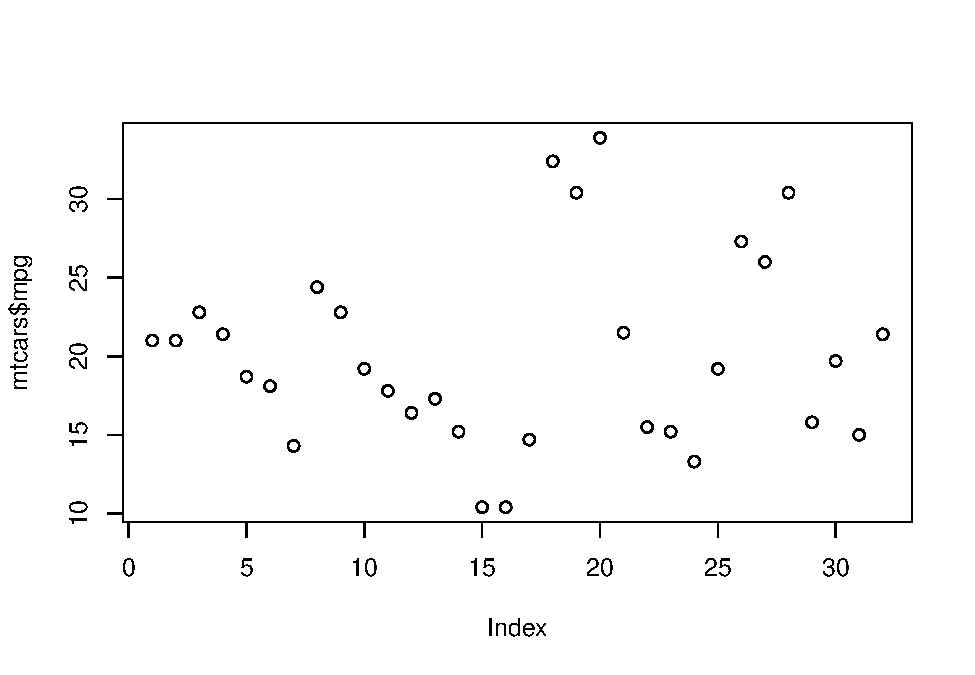
\includegraphics{210431461_CSC8639_Dissertation_files/figure-latex/fig2-1.pdf}
\caption{Another sample figure}
\end{figure}

You can use \textbf{bookdown} to allow references for Tables and
Figures.

\hypertarget{tables}{%
\subsection{Tables}\label{tables}}

Below we can see how to use tables.

See awesome Table\textasciitilde{}\ref{tab:table} which is written
directly in LaTeX in source Rmd file.

\begin{table}
 \caption{Sample table title}
  \centering
  \begin{tabular}{lll}
    \toprule
    \multicolumn{2}{c}{Part}                   \\
    \cmidrule(r){1-2}
    Name     & Description     & Size ($\mu$m) \\
    \midrule
    Dendrite & Input terminal  & $\sim$100     \\
    Axon     & Output terminal & $\sim$10      \\
    Soma     & Cell body       & up to $10^6$  \\
    \bottomrule
  \end{tabular}
  \label{tab:table}
\end{table}

You can also use R code for that.

\begin{Shaded}
\begin{Highlighting}[]
\NormalTok{knitr}\SpecialCharTok{::}\FunctionTok{kable}\NormalTok{(}\FunctionTok{head}\NormalTok{(mtcars), }\AttributeTok{caption =} \StringTok{"Head of mtcars table"}\NormalTok{)}
\end{Highlighting}
\end{Shaded}

\begin{longtable}[]{@{}lrrrrrrrrrrr@{}}
\caption{Head of mtcars table}\tabularnewline
\toprule
& mpg & cyl & disp & hp & drat & wt & qsec & vs & am & gear & carb \\
\midrule
\endfirsthead
\toprule
& mpg & cyl & disp & hp & drat & wt & qsec & vs & am & gear & carb \\
\midrule
\endhead
Mazda RX4 & 21.0 & 6 & 160 & 110 & 3.90 & 2.620 & 16.46 & 0 & 1 & 4 &
4 \\
Mazda RX4 Wag & 21.0 & 6 & 160 & 110 & 3.90 & 2.875 & 17.02 & 0 & 1 & 4
& 4 \\
Datsun 710 & 22.8 & 4 & 108 & 93 & 3.85 & 2.320 & 18.61 & 1 & 1 & 4 &
1 \\
Hornet 4 Drive & 21.4 & 6 & 258 & 110 & 3.08 & 3.215 & 19.44 & 1 & 0 & 3
& 1 \\
Hornet Sportabout & 18.7 & 8 & 360 & 175 & 3.15 & 3.440 & 17.02 & 0 & 0
& 3 & 2 \\
Valiant & 18.1 & 6 & 225 & 105 & 2.76 & 3.460 & 20.22 & 1 & 0 & 3 & 1 \\
\bottomrule
\end{longtable}

\hypertarget{lists}{%
\subsection{Lists}\label{lists}}

\begin{itemize}
\tightlist
\item
  Item 1
\item
  Item 2
\item
  Item 3
\end{itemize}

\hypertarget{refs}{}
\begin{CSLReferences}{0}{0}
\leavevmode\vadjust pre{\hypertarget{ref-data2017}{}}%
\CSLLeftMargin{{[}1{]} }
\CSLRightInline{Cabinet Office and Government Digital Service,
{``Government transformation strategy: Better use of data.''} HM
Government;
\url{https://www.gov.uk/government/publications/government-transformation-strategy-2017-to-2020/government-transformation-strategy-better-use-of-data},
2017.}

\leavevmode\vadjust pre{\hypertarget{ref-data2020}{}}%
\CSLLeftMargin{{[}2{]} }
\CSLRightInline{Department for Digital, Culture, Media \& Sport and
Department for Science, Innovation \& Technology, {``National data
strategy.''} HM Government;
\url{https://www.gov.uk/government/publications/uk-national-data-strategy/national-data-strategy},
2020.}

\leavevmode\vadjust pre{\hypertarget{ref-data2021}{}}%
\CSLLeftMargin{{[}3{]} }
\CSLRightInline{M. of Defence, {``Data strategy for defence,''}
\emph{GOV.UK}. HM Government;
\url{https://www.gov.uk/government/publications/data-strategy-for-defence/data-strategy-for-defence},
2021.}

\leavevmode\vadjust pre{\hypertarget{ref-data2022}{}}%
\CSLLeftMargin{{[}4{]} }
\CSLRightInline{Central Digital \& Data Office, {``Transforming for a
digital future: 2022 to 2025 roadmap for digital and data.''} HM
Government;
\url{https://www.gov.uk/government/publications/roadmap-for-digital-and-data-2022-to-2025/transforming-for-a-digital-future-2022-to-2025-roadmap-for-digital-and-data},
2022.}

\leavevmode\vadjust pre{\hypertarget{ref-trust}{}}%
\CSLLeftMargin{{[}5{]} }
\CSLRightInline{Centre for Data Ethics \& Innovation, {``Addressing
trust in public sector data use.''}
\url{https://www.gov.uk/government/publications/cdei-publishes-its-first-report-on-public-sector-data-sharing/addressing-trust-in-public-sector-data-use\#introduction--context}.}

\leavevmode\vadjust pre{\hypertarget{ref-pathway}{}}%
\CSLLeftMargin{{[}6{]} }
\CSLRightInline{Government Analysis Function, {``Types of data in
government learning pathway.''}
\url{https://analysisfunction.civilservice.gov.uk/learning-development/learning-pathways/types-of-data-in-government-learning-pathway/},
2022.}

\leavevmode\vadjust pre{\hypertarget{ref-onstool}{}}%
\CSLLeftMargin{{[}7{]} }
\CSLRightInline{Office for National Statistics, {``Time series
explorer.''}
\url{https://www.ons.gov.uk/timeseriestool?query=\&topic=\&updated=\&fromDateDay=\&fromDateMonth=\&fromDateYear=\&toDateDay=\&toDateMonth=\&toDateYear=\&size=50},
Unknown.}

\leavevmode\vadjust pre{\hypertarget{ref-TVStore}{}}%
\CSLLeftMargin{{[}8{]} }
\CSLRightInline{Y. An, Y. Su, Y. Zhu, and J. Wang, {``TVStore:
Automatically bounding time series storage via time-varying
compression,''} in \emph{Proceedings of the 20th USENIX conference on
file and storage technologies}, in USENIX conference on file and STorage
technologies. Santa Clara, CA, USA: USENIX Association, 2022, pp.
83--99.}

\leavevmode\vadjust pre{\hypertarget{ref-datapoint}{}}%
\CSLLeftMargin{{[}9{]} }
\CSLRightInline{J. Donckt, J. Donckt, M. Rademaker, and S. Hoecke,
{``Data point selection for line chart visualization: Methodological
assessment and evidence-based guidelines.''} 2023. doi:
\href{https://doi.org/10.48550/arXiv.2304.00900}{10.48550/arXiv.2304.00900}.}

\leavevmode\vadjust pre{\hypertarget{ref-Sveinn}{}}%
\CSLLeftMargin{{[}10{]} }
\CSLRightInline{S. Steinarsson, {``Downsampling time series for visual
representation.''} University of Iceland, Faculty of Industrial
Engineering, Mechanical Engineering; Computer Science, School of
Engineering; Natural Sciences, University of Iceland, Reykjavik,
Iceland, 2013.}

\leavevmode\vadjust pre{\hypertarget{ref-Shift}{}}%
\CSLLeftMargin{{[}11{]} }
\CSLRightInline{The Shift Project, {``Implementing digital
sufficiency,''} 2020.}

\leavevmode\vadjust pre{\hypertarget{ref-downsampling}{}}%
\CSLLeftMargin{{[}12{]} }
\CSLRightInline{W. Aigner, S. Miksch, W. Muller, H. Schumann, and C.
Tominski, {``Visual methods for analyzing time-oriented data,''}
\emph{IEEE Transactions on Visualization and Computer Graphics}, vol.
14, no. 1, pp. 47--60, 2008, doi:
\href{https://doi.org/10.1109/TVCG.2007.70415}{10.1109/TVCG.2007.70415}.}

\leavevmode\vadjust pre{\hypertarget{ref-sampling}{}}%
\CSLLeftMargin{{[}13{]} }
\CSLRightInline{B. C. Kwon, J. Verma, P. J. Haas, and C. Demiralp,
{``Sampling for scalable visual analytics,''} \emph{IEEE Computer
Graphics and Applications}, vol. 37, no. 1, pp. 100--108, 2017, doi:
\href{https://doi.org/10.1109/MCG.2017.6}{10.1109/MCG.2017.6}.}

\leavevmode\vadjust pre{\hypertarget{ref-MinMaxLTTB}{}}%
\CSLLeftMargin{{[}14{]} }
\CSLRightInline{J. Donckt, J. Donckt, M. Rademaker, and S. Hoecke,
{``MinMaxLTTB: Leveraging MinMax-preselection to scale LTTB.''} 2023.
Available: \url{https://arxiv.org/abs/2305.00332}}

\leavevmode\vadjust pre{\hypertarget{ref-imputeTS_R}{}}%
\CSLLeftMargin{{[}15{]} }
\CSLRightInline{S. Moritz and T. Bartiz-Beielstein, {``imputeTS: Time
series missing value imputation in r,''} vol. 9.1. R Journal, 2017. doi:
\href{https://doi.org/10.32614/RJ-2017-009}{10.32614/RJ-2017-009}.}

\leavevmode\vadjust pre{\hypertarget{ref-catch22_R}{}}%
\CSLLeftMargin{{[}16{]} }
\CSLRightInline{C. H. Lubba, B. Fulcher, T. Henderspn, B. Harris, O. r.
TL, and O. Cliff, {``catch22: CAnonical time-series CHaracteristics.''}
R Journal, 2022. doi:
\href{https://doi.org/10.5281/zenodo.6673597}{10.5281/zenodo.6673597}.}

\leavevmode\vadjust pre{\hypertarget{ref-political_transparency}{}}%
\CSLLeftMargin{{[}17{]} }
\CSLRightInline{K. E. Levy and D. M. Johns, {``When open data is a
trojan horse: The weaponization of transparency in science and
governance,''} \emph{Big Data \& Society}, vol. 3, no. 1, 2016, doi:
\href{https://doi.org/10.1177/2053951715621568}{10.1177/2053951715621568}.}

\leavevmode\vadjust pre{\hypertarget{ref-social_transparency}{}}%
\CSLLeftMargin{{[}18{]} }
\CSLRightInline{J. Bates, H. Kennedy, I. Medina Perea, S. Oman, and L.
Pinney, {``Socially meaningful transparency in data-based systems:
Reflections and proposals from practice,''} \emph{Journal of
Documentation}, vol. ahead--of--print, 2023, doi:
\href{https://doi.org/10.1108/JD-01-2023-0006}{10.1108/JD-01-2023-0006}.}

\leavevmode\vadjust pre{\hypertarget{ref-transparency_lack}{}}%
\CSLLeftMargin{{[}19{]} }
\CSLRightInline{M. Ananny and K. Crawford, {``Seeing without knowing:
Limitations of the transparency ideal and its application to algorithmic
accountability,''} \emph{New Media \& Society}, vol. 20, no. 3, pp.
973--989, 2018, doi:
\href{https://doi.org/10.1177/1461444816676645}{10.1177/1461444816676645}.}

\leavevmode\vadjust pre{\hypertarget{ref-digital_transparency}{}}%
\CSLLeftMargin{{[}20{]} }
\CSLRightInline{R. Matheus, M. Janssen, and T. Janowski, {``Design
principles for creating digital transparency in government,''}
\emph{Government Information Quarterly}, vol. 38, no. 1, 2021, doi:
\url{https://doi.org/10.1016/j.giq.2020.101550}.}

\leavevmode\vadjust pre{\hypertarget{ref-transparency_obfuscation}{}}%
\CSLLeftMargin{{[}21{]} }
\CSLRightInline{N. A. Draper and J. Turow, {``The corporate cultivation
of digital resignation,''} \emph{New Media \& Society}, vol. 21, no. 8,
pp. 1824--1839, 2019, doi:
\href{https://doi.org/10.1177/1461444819833331}{10.1177/1461444819833331}.}

\leavevmode\vadjust pre{\hypertarget{ref-transparency_fallacy}{}}%
\CSLLeftMargin{{[}22{]} }
\CSLRightInline{J. A. Obar, {``Sunlight alone is not a disinfectant:
Consent and the futility of opening big data black boxes (without
assistance),''} \emph{Big Data \& Society}, vol. 7, no. 1, 2020, doi:
\href{https://doi.org/10.1177/2053951720935615}{10.1177/2053951720935615}.}

\leavevmode\vadjust pre{\hypertarget{ref-timenotes}{}}%
\CSLLeftMargin{{[}23{]} }
\CSLRightInline{J. Walker, R. Borgo, and MW. Jones, {``TimeNotes: A
study on effective chart visualization and interaction techniques for
time-series data,''} \emph{IEEE Transactions on Visualization and
Computer Graphics}, vol. 22, 2016, doi:
\href{https://doi.org/10.1109/TVCG.2015.2467751}{10.1109/TVCG.2015.2467751}.}

\leavevmode\vadjust pre{\hypertarget{ref-plotly}{}}%
\CSLLeftMargin{{[}24{]} }
\CSLRightInline{J. Donckt, J. Donckt, E. Deprost, and S. Hoecke,
{``Plotly-resampler: Effective visual analytics for large time
series,''} \emph{IEEE Visualization and Visual Analytics}, 2022, doi:
\href{https://doi.org/10.1109/VIS54862.2022.00013}{10.1109/VIS54862.2022.00013}.}

\leavevmode\vadjust pre{\hypertarget{ref-imputeTS}{}}%
\CSLLeftMargin{{[}25{]} }
\CSLRightInline{S. Moritz and T. Bartiz-Beielstein, {``imputeTS: Time
series missing value imputation in r.''} R Journal, 2017. Available:
\url{https://cran.r-project.org/web/packages/imputeTS/vignettes/imputeTS-Time-Series-Missing-Value-Imputation-in-R.pdf}}

\leavevmode\vadjust pre{\hypertarget{ref-storage}{}}%
\CSLLeftMargin{{[}26{]} }
\CSLRightInline{A. Visheratin \emph{et al.}, {``Peregreen {\textendash}
modular database for efficient storage of historical time series in
cloud environments,''} in \emph{2020 USENIX annual technical conference
(USENIX ATC 20)}, USENIX Association, 2020, pp. 589--601. Available:
\url{https://www.usenix.org/conference/atc20/presentation/visheratin}}

\leavevmode\vadjust pre{\hypertarget{ref-CatchUp}{}}%
\CSLLeftMargin{{[}27{]} }
\CSLRightInline{T. Schlossnagle, J. Sheehy, and C. McCubbin,
{``Always-on time-series database: Keeping up where there's no way to
catch up,''} \emph{Commun. ACM}, vol. 64, no. 7, pp. 50--56, 2021,
Available: \url{https://doi.org/10.1145/3442518}}

\leavevmode\vadjust pre{\hypertarget{ref-climate}{}}%
\CSLLeftMargin{{[}28{]} }
\CSLRightInline{I. Foster \emph{et al.}, {``Computing just what you
need: Online data analysis and reduction at extreme scales,''} in
\emph{Euro-par 2017}, F. F. Rivera, T. F. Pena, and J. C. Cabaleiro,
Eds., in Lecture notes in computer science (including subseries lecture
notes in artificial intelligence and lecture notes in bioinformatics).
Germany: Springer Verlag, 2017, pp. 3--19. doi:
\href{https://doi.org/10.1007/978-3-319-64203-1_1}{10.1007/978-3-319-64203-1\_1}.}

\leavevmode\vadjust pre{\hypertarget{ref-dashql}{}}%
\CSLLeftMargin{{[}29{]} }
\CSLRightInline{A. Kohn, D. Moritz, and T. Neumann, {``DashQL --
complete analysis workflows with SQL.''} 2023. doi:
\href{https://doi.org/10.48550/arXiv.2306.03714}{10.48550/arXiv.2306.03714}.}

\leavevmode\vadjust pre{\hypertarget{ref-EveryNth}{}}%
\CSLLeftMargin{{[}30{]} }
\CSLRightInline{U. Jugel, Z. Jerzak, G. Hackenbroic, and V. Markl,
{``VDDA: Automatic visualization-driven data aggregation in relational
databases,''} \emph{The VLDB Journal}, vol. 25, 2016, doi:
\href{https://doi.org/10.1007/s00778-015-0396-z}{10.1007/s00778-015-0396-z}.}

\leavevmode\vadjust pre{\hypertarget{ref-MinMaxOrdered}{}}%
\CSLLeftMargin{{[}31{]} }
\CSLRightInline{W. Yunhai \emph{et al.}, {``OM3: An ordered multi-level
min-max representation for interactive progressive visualization of time
series,''} in \emph{Proc. ACM manag. data}, ACM, 2023. Available:
\url{https://doi.org/10.1145/3589290}}

\leavevmode\vadjust pre{\hypertarget{ref-M4}{}}%
\CSLLeftMargin{{[}32{]} }
\CSLRightInline{U. Jugel, Z. Jerzak, G. Hackenbroich, and V. Markl,
{``M4: A visualization-oriented time series data aggregation.
Proceedings of the VLDB endowment,''} vol. 7, 2014, Available:
\url{https://www.vldb.org/2014/program/http://www.vldb.org/pvldb/vol7/p797-jugel.pdf}}

\leavevmode\vadjust pre{\hypertarget{ref-catch22}{}}%
\CSLLeftMargin{{[}33{]} }
\CSLRightInline{C. H. Lubba, S. S. Sarab, P. Knaute, S. R. Schultz, B.
D. Fulcher, and N. S. Jones, {``catch22: CAnonical time-series
CHaracteristics,''} \emph{Data Mining and Knowledge Discovery}, vol. 33,
2019, doi:
\href{https://doi.org/10.1007/s10618-019-00647-x}{10.1007/s10618-019-00647-x}.}

\leavevmode\vadjust pre{\hypertarget{ref-fulcher2017}{}}%
\CSLLeftMargin{{[}34{]} }
\CSLRightInline{B. D. Fulcher and N. S. Jones, {``Highly comparative
feature-based time-series classification,''} \emph{IEEE Transactions on
Knowledge and Data Engineering}, vol. 26, no. 12, pp. 3026--3037, 2014,
doi:
\href{https://doi.org/10.1109/TKDE.2014.2316504}{10.1109/TKDE.2014.2316504}.}

\leavevmode\vadjust pre{\hypertarget{ref-bagnall}{}}%
\CSLLeftMargin{{[}35{]} }
\CSLRightInline{A. Bagnall, J. Lines, A. Bostrom, J. Large, and E.
Keogh, {``The great time series classification bake off: A review and
experimental evaluation of recent algorithmic advances,''} \emph{Data
Mining and Knowledge Discovery}, vol. 31, 2017, doi:
\href{https://doi.org/10.1007/s10618-016-0483-9}{10.1007/s10618-016-0483-9}.}

\leavevmode\vadjust pre{\hypertarget{ref-henderson}{}}%
\CSLLeftMargin{{[}36{]} }
\CSLRightInline{T. Henderson and B. D. Fulcher, {``An empirical
evaluation of time-series feature sets,''} in \emph{2021 international
conference on data mining workshops (ICDMW)}, 2021, pp. 1032--1038. doi:
\href{https://doi.org/10.1109/ICDMW53433.2021.00134}{10.1109/ICDMW53433.2021.00134}.}

\end{CSLReferences}

\bibliographystyle{unsrt}
\bibliography{references.bib}


\end{document}
